\section{Haiku OS}

\subsection{Nombre del proyecto o sistema operativo}
Según \citep{leavengood2012haiku}, Haiku Os es un proyecto visionario con el nombre del sistema operativo Haiku OS en la actualidad,pero que antes era OpenBeOS, un sistema operativo fundada en la División de Corporaciones del Estado de Nueva York como una organización sin fines de lucro en julio del 2003. por su fundador Michael Phipps.
El nombre del sistema operativo proviene de la palabra japoness ``Haiku``, por que era usada en los mensajes de error de BeOS, eran mensajes presentados de forma poética japonesa.

\subsection{Enlace al repositorio y/o documentación oficial}
\begin{itemize}
    \item \textbf{Repositorio oficial (espejo en GitHub):} \url{https://github.com/haiku/haiku} — funciona como un \textit{mirror} del repositorio principal alojado en el servidor de Haiku, donde se gestiona el desarrollo activo del sistema operativo. (Haiku Project)
    \item \textbf{Repositorio principal (Gerrit):} \url{https://review.haiku-os.org/haiku} — servidor oficial utilizado para la revisión y aprobación del código fuente. (Haiku Project)
    \item \textbf{Sitio web oficial del proyecto:} \url{https://www.haiku-os.org/get-haiku/installation-guide/}
\end{itemize}


\subsection{Objetivo del proyecto}
Este sistema operativo tiene varios objetivo, dentro de las claves se encuentran:
\begin{itemize}
    \item \textbf{Facil de usar y sencillez:} Según \citep{haiku_website_2025} El desarrollo de Haiky OS inspirado en BeOS, fue diseñado para la informática personal, Haiku OS es rápido, fácil de aprender y muy potente. Accesible por cualquier usuario que tenga a su alcance.
    El desarrollo se centra en la informática personal y multimedia \citep{Gonzales2017haiku}. 
    \item \textbf{Alto rendimiento y respuesta rápida:} Al igual que BeOS, por la potencia de lo microprocesadores. Capaz de aprovechar cuatro o mas procesadores, BeOS se basa en el multiprocesamiento simétrica que acelera las operaciones \citep{beinc_beos_datasheet}. Haiku mantenío esa velocidad, respuestas y potencia. Como menciona Leavengood en \citep{leavengood2012haiku}, Haiku OS  y BeOS son capaz de manejar múltiples tareas y procesos. y según \citep{Installing2024haiku} Dado que esta inspirada en BeFS(BeFiles System), lo permite que aumente la velocidad de acceso a los datos y almacenamiento.
    \item \textbf{Código abierto y comunidad activa:} Haiku OS es un proyecto de código abierto, lo que significa que su código fuente está disponible para que cualquier usuario pueda revisarlo, modificarlo y mejorar su desarrollo \citep{leavengood2012haiku}.
    \item \textbf{Compatibilidad con aplicaciones de BeOS:} Haiku OS busca mantener la compatibilidad con las aplicaciones desarrolladas para BeOS, lo que permite a los usuarios ejecutar software antiguo en el nuevo sistema operativo \citep{Gonzales2017haiku}.
    \item \textbf{Arquitectura modular} Haiku OS está adopta el kernel hibrido multihilo, lo que le permite organizar de manera eficiente todas las tareas  y procesos. El sistema operativo se basa en principios de modularidad donde los componentes se pueden mejorar o reemplazarse sin afectar al sistema \citep{tutorialspoint_haiku_os}.
\end{itemize}
\subsection{Lenguaje(s) de implementación}
Haiku esta implementado en C++, haciendo uso de una API de Be orientada a objetos (The kits) que facilita el desarrollo de aplicaciones y controladores de dispositivos \citep{leavengood2012haiku}.
incluye contenedores de la Biblioteca de Plantillas Estandar de C++ (STL) y otras bibliotecas de terceros como OpenSSL, SQLite y zlib \citep{haiku_website_2025}.
\subsection{Arquitectura del sistema (monolítica, microkernel, etc.)}
El sistema operativo esta basado en BeOS un Kernel hibrido modular. Su núcleo se desarrollo de una rama de NewOS, la modularidad permite a los controladores y otros componentes que se carguen de manera dinamica todo lo proceso segun sea necesario. 
La siguientes son las capas principales que conforman el sistema operativo, según \citep{2025deployment}:
\begin{itemize}
    \item  \textbf{Capa de nucleo: } El nucleo de NewOS sirve para servicio como: multitarea, gestión de memoria, controladores y administrador de archivos. 
    \item \textbf{Servidor de aplicaciones: } El servido de aplicaciones gestiona las ventanas, el dibujo y el renderizado. Esta diseñado para un alto rendimiento y se integra con el servidor de entrada y el kit de herramientas.
    \item \textbf{Gestión de paquetes: } Haiku es compatible con Be File System (BFC) que incluye atributos de archivos extendidos.
    \item \textbf{Controlador de red:} Haiku incluye una pila de red modular compatible con estaciones.
\end{itemize}
En la siguiente imagen es al arquitectura del sistema operativo BeOS. Se puede observar que entre el hardware y las aplicaciones del software se encuentra el software BeOS. El software del sistema operativo tiene 3 capas, capa de micronucleo, capa de servidor y capa de software.
\begin{figure}[H]
\centering
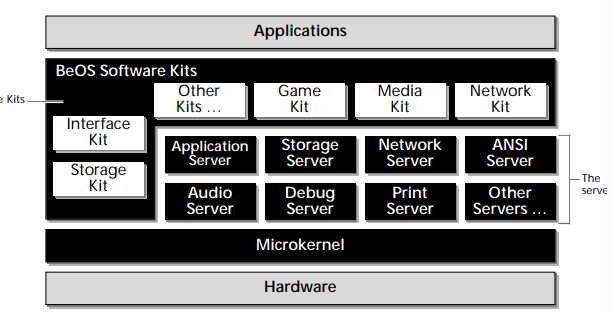
\includegraphics[width=1\textwidth]{figures/ArquitecturaBeos.png}
\centering
\caption{Arquitectura del sistema operativo BeOS.}
\label{fig:arquitecturaBeOS}
\centering
\small Fuente: Obtenido de \citep{beinc_beos_bible_kits} 
\end{figure}

\begin{table}[H]
\centering
\caption{Comparación entre tipos de kernel: Monolítico, Microkernel e Híbrido/Modular (Haiku OS)}
\label{tab:kernel_comparacion}
\begin{tabular}{|p{2.5cm}|p{4.2cm}|p{4.2cm}|p{4.2cm}|}
\hline
\textbf{Aspecto} & \textbf{Monolítico} & \textbf{Microkernel} & \textbf{Híbrido/Modular} \\ \hline

\textbf{Definición} &
Incluye todos los servicios(gestión de memoria, E/S, controladores). &
Separa los servicios en procesos de usuario y nucleo(planificación, IPC, memoria). &
Combina elementos de ambos modelos. \\ \hline

\textbf{Arquitectura} &
Comunicación directa entre subsistemas. &
Diseño con fuerte aislamiento y comunicación por mensajes. &
Diseño que usa comunicación interna. \\ \hline

\textbf{Rendimiento} &
Muy alto.&
Menor rendimiento por la sobrecarga del IPC. &
Similar al monolítico. \\ \hline

\textbf{Estabilidad y seguridad} &
Baja: Debido a fallos en un módulo. &
Alta: los fallos no afectan al núcleo principal. &
Intermedia: mayor aislamiento que el monolítico. \\ \hline

\textbf{Mantenibilidad} &
Difícil de mantener y depurar; requiere recompilar el núcleo completo. &
Alta: componentes independientes facilitan depuración y portabilidad. &
Moderada: estructura modular permite reemplazar componentes sin reconstruir todo el sistema. \\ \hline

\textbf{Sistemas Operativos} &
Linux, FreeBSD, Unix clásico. &
MINIX3, QNX, seL4, Mach. &
Windows NT, macOS (XNU), Haiku OS, BeOS. \\ \hline

\end{tabular}
\centering
\small Fuente: Adaptado de \citep{tanenbaum2015modern, herder2009minix3, russinovich2012windows, haiku2023arch, windriver2008osarch}.
\end{table}

\subsection{Componentes implementados (procesos, memoria, archivos, etc.)}


\subsection{Herramientas utilizadas (compiladores, emuladores, etc.)}


\subsection{Nivel de complejidad y accesibilidad para estudiantes}
